%% ------------------------------------------------------------------------- %%
\chapter{Planejamento do Estudo}
\label{cap:planejamento}

Conforme discutido no Capítulo \ref{cap:trabalhos-relacionados}, muitos 
trabalhos avaliaram TDD, e alguns deles relatam inclusive uma melhora
no design de classes, como um menor acoplamento, uma maior coesão, e até mesmo
mais simplicidade. 
Grande parte deles focam nos efeitos da prática
no código final, mas poucos estudos tentam entender a possível influência da experiência
nos resultados encontrados e como TDD e a
prática de escrever o teste antes do código real realmente guiam o programador 
em direção à essas melhorias.

Para entendê-las, este trabalho propõe um estudo qualitativo com 
desenvolvedores praticantes de TDD atuantes em empresas de desenvolvimento de
software. Este capítulo detalha o planejamento do experimento, 
bem como o processo de análise dos dados colhidos.

%% ------------------------------------------------------------------------- %%
\section{Design da pesquisa}

Baseando-se no fato de que o processo de desenvolvimento de software envolve 
diversos fatores humanos e é totalmente sensível ao contexto em que ele está 
inserido, este trabalho faz uso de métodos qualitativos de pesquisa para a coleta e 
análise dos dados.

Os participantes serão separados em diferentes grupos, de acordo com sua
experiência em desenvolvimento de software e com a prática de TDD. Os níveis
irão variar de pessoas sem experiência até pessoas com experiência em ambas
as categorias citadas anteriormente.
Todos os participantes serão
solicitados a resolver alguns problemas utilizando Java, dentro de um
período de tempo limitado. Alguns desses grupos deverão
utilizar TDD durante o processo de desenvolvimento. Todas as implementações,
além de salvas, serão filmadas para que o desenvolvedor tenha acesso futuro
a cada passo tomado durante a implementação.
Ao final do exercício,
todos responderão um questionário.

Uma análise inicial servirá para filtrar os candidatos
mais interessantes, que serão posteriormente entrevistados. 
Todos os dados gerados no processo,
como código produzido e as entrevistas, serão analisados e darão origem
à seção de resultados encontrados.

A intenção deste estudo é obter informações relevantes sobre como os
praticantes de TDD utilizam a prática para influenciar o design de suas
classes. Na tentativa de capturar o máximo de informações possíveis, esse estudo
inclui análises dos códigos produzidos e das entrevistas com os participantes.

%% ------------------------------------------------------------------------- %%
\subsection{Participantes da pesquisa}
\label{sec:planejamento-participantes}

Desenvolvedores atuantes no mercado de 
software brasileiro serão selecionados para participarem da pesquisa.
Certos critérios foram levados em consideração no momento de convidar desenvolvedores:

\begin{itemize}
	\item \textbf{Experiência em TDD.} O estudo convidará praticantes com diferentes
	níveis de experiência. Programadores inexperientes em TDD (sem conhecimentos teóricos e práticos)
	e programadores com experiência em TDD (praticantes a no mínimo 3 anos)
	
	\item \textbf{Experiência em desenvolvimento de software.} Participantes
	experientes (com no mínimo 3 anos de desenvolvimento e bons conhecimentos em orientação a objetos) e 
	inexperientes (com no máximo 1 ano de desenvolvimento e algum conhecimento de orientação a objetos).

	\item \textbf{Localizados em São Paulo (SP).} Para facilitar a execução do exercício
	e o processo de entrevista, já que o pesquisador encontra-se em São Paulo;

	\item \textbf{Experiência em Java.} 
	Participantes devem ter experiência em Java, já que os problemas deverão ser resolvidos
	nessa linguagem.	
\end{itemize}

%% ------------------------------------------------------------------------- %%
\subsection{Agrupamento dos Participantes}

Os participantes serão agrupados em grupos, separados por experiência em desenvolvimento
de software, experiência em TDD, e se o grupo utilizará TDD ou não. A tabela abaixo
descreve os grupos:

\begin{table}
	\caption{Participantes e os diferentes grupos}
	\begin{tabular}{c | c | c | c |}
		\hline
		Grupo & Experiência em Desenvolvimento de Software & Experiência em TDD & Fará TDD? \\ 	\hline
		1 & Sim & Sim & Sim \\ 	\hline
		2 & Sim & Sem & Sim \\ 	\hline
		3 & Sim & Sem & Não \\ 	\hline
		4 & Sim & Sim & Não \\ 	\hline
		5 & Não & Não & Sim \\ 	\hline
	\end{tabular}
\end{table}

O objetivo desses grupos é conseguir isolar alguns dos principais fatores de influência,
e entender a atuação da prática de TDD em cada um desses grupos. Mais especificamente,
cada um dos grupos podem revelar informações interessantes como:

\begin{itemize}
	\item \textbf{Grupo 1:} Por ser composto de participantes com experiência tanto
	em desenvolvimento de software quanto em TDD, deve-se entender o porquê de
	pessoas com tanta experiência optam por utilizar a prática;
	
	\item \textbf{Grupo 2 e 3:} Por serem participantes com experiência em desenvolvimento
	de software, mas não praticantes de TDD, deve-se entender a diferença entre
	praticar TDD e não praticar TDD;
	
	\item \textbf{Grupo 4:} Por terem ambas experiências e não praticarem TDD durante o estudo,
	existem duas possibilidades a serem discutidas: caso o código produzido seja de qualidade, 
	deve-se entender o porquê isso aconteceu e o motivo de TDD não ter sido necessário; 
	caso o código produzido seja de menor qualidade, o resultado coincide com o encontrado na
	literatura;
	
	\item \textbf{Grupo 5:} Por serem participantes sem nenhuma experiência, é esperado que
	a prática ajude na qualidade do código. Caso isso não aconteça, deve-se entender o motivo de TDD
	não ter auxiliado os desenvolvedores durante a criação do design.
\end{itemize}

%% ------------------------------------------------------------------------- %%
\subsection{Execução do estudo}
\label{sec:execucao}	

Todos os participantes serão convidados a comparecer em um laboratório pré-definido,
com todos os softwares já instalados e prontos para o início do estudo. Todos eles
terão acesso aos enunciados dos problemas, discutidos na
Seção \ref{sec:exercicios}.

Os participantes terão 2h para resolver os exercícios. 
Todos os códigos deverão ser salvos ao final do estudo para que possam ser analisado juntos
com os dados da entrevista.
O tempo é considerado suficiente
para que o participante resolva todos eles. Em caso do tempo acabar antes do participante
terminar todos os exercícios, isso será levado em conta no momento da entrevista e nos
dados colhidos desse participante.

Os participantes não poderão se comunicar durante o exercício, e cada um deles receberá
os exercícios em ordens diferentes, para tentar diminuir o fator de aprendizado que 
pode ocorrer durante a resolução dos problemas.

Ao final, todos deverão responder a um questionário online, que fará perguntas sobre a qualidade
do código que ele acabou de produzir. Esses questionários serão diferentes de acordo com o 
grupo do participante e são melhor detalhados na Seção \ref{sec:questionario}

%% ------------------------------------------------------------------------- %%
\subsection{Problemas Propostos}
\label{sec:exercicios}

Serão propostos 4 problemas que devem ser resolvidos pelos participantes, utilizando
linguagem Java. Participantes que praticarão TDD utilizarão JUnit \footnote{\url{http://www.junit.org}. Último acesso em 18 de Julho de 2011} 
para a escrita de testes
automatizados de unidade. O objetivo desses exercícios é simular problemas de design 
recorrentes em diversos projetos de software.  Os enunciados encontram no Apêndice 
\ref{ape:exercicios}.

O primeiro exercício pede ao participante que implemente uma calculadora de salário, onde
o algoritmo de cálculo varia de acordo com o cargo do funcionário. Em uma implementação
procedural e mais difícil de ser mantida, esse problema seria resolvido através de uma
sequência de "ifs"; todo novo cargo obrigaria o desenvolvedor a acrescentar mais um "if" 
nessa classe. Uma implementação mais flexível teria cada algoritmo de cálculo em uma 
classe separada.

O segundo exercício pede que o participante implemente o processo de geração de uma nota fiscal e, após
esse processo, a nota gerada deve passar por diversos outros processos, como envio por e-mail, envio
para um sistema terceiro, persistir na base de dados, e etc. Possíveis más implementações incluem a 
implementação de uma única classe que faria todo o processo, ou uma classe altamente acoplada.
Uma solução mais elegante seria extrair cada responsabilidade em uma classe diferente e compô-las
através de, por exemplo, a implementação do padrão Observer \cite{gof}.

O terceiro exercício pede ao participante a implementação que um simples processador de boletos que
deve marcar a fatura como paga, caso a soma de pagamentos seja maior ou igual ao valor da fatura. 
Em uma implementação elegante, o comportamento de marcar a fatura como paga deveria ficar dentro
da classe "Fatura", ou entidade similar criada pelo participante.

O quarto exercício dá ao participante um algoritmo matemático qualquer e pede que ele altere a saída
do programa. Por ser uma outra responsabilidade, esse código deveria estar em uma outra classe, específica,
e não dentro da classe que contém o algoritmo.

%% ------------------------------------------------------------------------- %%
\subsection{Gravação da implementação}
\label{sec:planejamento-gravacao}

A tela do computador do participante durante a implementação será gravada. 
O objetivo da gravação é possibilitar o pesquisador a encontrar informações
sobre a frequência que o desenvolvedor volta ao teste para avaliar mudanças de ideia sobre
nomes, parâmetros, tipos de retorno e exceções lançadas por métodos, ou nomes
e responsabilidades de classes.

Muito do que a literatura diz sobre os efeitos de TDD no teste é baseado
na relação entre um código difícil de ser testado isoladamente e a má aplicação
de princípios de orientação a objetos. A gravação ajudará a mostrar se o teste
realmente alarma o desenvolvedor em relação a esses princípios.

%% ------------------------------------------------------------------------- %%
\subsection{Questionário}
\label{sec:questionario}

Como mencionado anteriormente, ao final dos exercícios o participante responderá um questionário. 
O mesmo será diferenciado, de acordo com o grupo em que o participante se encaixa. Algumas
perguntas serão abertas, onde o participante poderá dar uma opinião mais profunda sobre o assunto,
e outras serão fechadas, onde ele deverá escolher um valor dentro de uma escala. A escala utilizada
será baseada na escala Likert e conterá os seguintes valores: concordo fortemente, concordo, não tenho certeza,
não concordo, não concordo fortemente.

As perguntas abaixo visam obter a opinião dos participantes sobre o estudo, como clareza dos
exercícios. O objetivo é aumentar a validade do estudo.
Além disso, entender se os exercícios propostos eram parecidos com os problemas encontrados no mundo
real ajudarão a aumentar a possibilidade de generalização do estudo. As perguntas abaixo deverão
ser feitas para todos os grupos:

\begin{enumerate}
	\item O entendimento dos exercícios estavam perfeitamente claros.
	\item Você teve tempo suficiente para resolver os exercícios.
	\item Você achou que os problemas de código e design enfrentados nos exercícios se parecem com os do mundo real.
\end{enumerate}

Na próxima bateria de perguntas, o objetivo é obter a visão do desenvolvedor sobre o próprio código gerado e como ele
faz para obter feedback sobre a qualidade do código que escreve. Também serão feitas para todos os grupos:

\begin{enumerate}
	\item Você acha que o código que você gerou é de fácil manutenção, ou seja, é um código fácil de mudar? Explique sua resposta.
	\item Durante a implementação, o que você fez para que o código saísse com um bom design?
	\item Acredita que alguma outra prática possa ajudar o desenvolvedor a criar um bom design? Quais? Por que?
\end{enumerate}

Para os grupos que utilizarão TDD, informações sobre a maneira com que a prática foi utilizada e a possível
diferença que ela fez serão requisitadas:

\begin{enumerate}
	\item Usei TDD o tempo todo, ou seja, sempre escrevi um teste antes de implementar, e tentei ser o mais simples possível.
	\item TDD fez alguma diferença na qualidade do código gerado? Explique sua resposta.
	\item A escrita de testes de unidade antes faz alguma diferença? Qual diferença? Explique sua resposta.
	\item Muitas pessoas dizem que TDD tem efeitos positivos no design. Você acredita nisso? Explique sua resposta.
	\item Os mesmos efeitos que a literatura diz sobre TDD no design não poderiam ser conseguidos também sem a utilização da prática? Explique sua resposta.
\end{enumerate}

%% ------------------------------------------------------------------------- %%
\subsection{Escolha de candidatos para a entrevista}

Após a implementação, os dados colhidos serão parcialmente analisados. O intuito
é encontrar, dentre todos os participantes, aqueles com dados mais relevantes
e que mereçam ser aprofundados.
Para isso, informações como qualidade dos códigos gerados, grupo que participa
dentro do estudo, e respostas no questionário influenciarão na escolha.

Após a escolha dos candidatos, os mesmos serão convidados a participar de
uma entrevista, objetivando entender melhor como a prática ou não de TDD
influenciou no design gerado.

%% ------------------------------------------------------------------------- %%
\subsection{Entrevistas}
\label{sec:planejamento-estrategia-entrevistas}

A entrevista será semi-estruturada, dando liberdade ao
pesquisador para mudar o rumo das perguntas, caso se faça necessário.
Além disso, todas as perguntas serão abertas, permitindo que o desenvolvedor dê
uma resposta ampla sobre o assunto. A Tabela \ref{tab:questoes} mostra a
relação entre os objetivos da entrevista e as perguntas formuladas no roteiro de
entrevista, encontrado no apêndice \ref{ape:entrevista} deste trabalho.

\begin{table}[h!]
	\begin{tabular}{ | p{6cm} | p{7cm} | p{2cm} | }
		\hline
		\textbf{Caracterizar a experiência do programador com desenvolvimento de
		software, boas práticas de desenvolvimento e TDD} 
		&
		Importante para caracterizar o público-alvo da pesquisa.
		&
		Seções \ref{entrevista:dados-basicos}, \ref{entrevista:caracterizacao}
		\\

		\hline
		\textbf{A relação entre a experiência do programador e os efeitos de TDD
		na qualidade do design} 
		&
		Por ser um possível fator de influência, o pesquisador colherá
		informações sobre a experiência do programador com desenvolvimento de software, 
		conceitos de orientação a objetos e TDD.
		&
		Seções \ref{entrevista:experiencia}
		\\

		\hline
		\textbf{A influência da utilização de TDD
	junto com outras práticas ágeis, como programação pareada, sobre o design} 
		&
		Por ser um outro possível fator de influência, o pesquisador colherá informações
		para diferenciar efeitos da programação pareada dos efeitos de TDD.
		&
		Seções \ref{entrevista:tdd-e-praticas-ageis}
		\\

		\hline
		\textbf{A visão do desenvolvedor sobre a prática de TDD} 
		&
		O pesquisador alinhará as definições da prática com todos os participantes da
		pesquisa.
		&
		Seções \ref{entrevista:pratica}
		\\

		\hline
		\textbf{Os efeitos de TDD sobre o acoplamento e a coesão geral das classes do
		sistema} 
		&
		Entender a opinião do participante sobre os efeitos de TDD
		nesses dois pontos importantes em sistemas orientados a objetos.
		&
		Seções \ref{entrevista:acoplamento}, \ref{entrevista:coesao}
		\\

		\hline
		\textbf{Como o desenvolvedor utiliza o feedback dos testes para guiar o
		design} 
		&
		Entender como o desenvolvedor utiliza os testes para melhorar o design
		e, para isso o pesquisador perguntará desde questões conceituais até questões
		bem práticas com discussões de trechos de código.
		&
		Seções \ref{entrevista:acoplamento}, \ref{entrevista:coesao}
		\\

		\hline
		\textbf{A visão do programador sobre a simplicidade que TDD agrega ao
		processo} 
		&
		Entender como TDD leva o programador à criação de códigos mais simples.
		&
		Seções \ref{entrevista:simplicidade}
		\\
		
		\hline												
	\end{tabular}
	\caption{Relação entre os objetivos e as perguntas da entrevista}
	\label{tab:questoes}
\end{table}

O processo de entrevista será composto por uma breve introdução da pesquisa, tomando
o cuidado para não enviesar o participante, seguida de algumas perguntas que visam
caracterizar o perfil do participante; perguntas como qual a experiência do
desenvolvedor em desenvolvimento de software e TDD são necessárias para ajudar o
pesquisador no entendimento das respostas dadas. Além disso, perguntas sobre
referências, livros e outros pontos de informação nas quais o participante lê a
respeito da prática servem para que o programador entenda o embasamento teórico
do praticante sobre TDD.

Em seguida, o pesquisador perguntará os principais pontos da pesquisa.
Para isso, o pesquisador fará uso não só de perguntas abertas, mas também
solicitará exemplos de código, para que as respostas se tornem técnicas e
específicas, caso necessário. O pesquisador solicitará ao participante que rascunhe pequenos
trechos de código durante a discussão, e essas anotações serão anexadas junto ao
conjunto de dados coletados da pesquisa.
Por fim, o pesquisador pedirá referências ao pesquisador sobre
possíveis próximos entrevistados, a fim de descobrir os programadores referencias 
na prática para aquele determinado participante.

Já que as decisões tomadas por um programador durante a atividade de design
pode ser influenciado por vários diferentes fatores, 
as perguntas serão feitas de modo que o participante deverá triangular suas respostas,
e tentar isolar o máximo possível a atividade de TDD dos outros possíveis fatores
de influência. Participantes que não articularem bem suas respostas serão eliminados
durante o processo de análise.

Todas as entrevistas serão gravadas, para que o pesquisador possa fazer a
transcrição e rever os dados a qualquer momento durante o processo. Além disso,
o pesquisador também tomará notas, capturando informações como reações dos 
participantes a determinadas perguntas, ou qualquer outra informação relevante. 

As entrevistas serão feitas em dias diferentes para que, ao final
de cada dia, o pesquisador possa discutir sobre os pontos levantados no dia
corrente e sugerir melhorias no instrumento de pesquisa. 

%% ------------------------------------------------------------------------- %%
\subsection{Avaliação do Especialista}
\label{sec:planejamento-especialista}

Um especialista será convidado a analisar os códigos-fonte e categorizá-los
em 3 categorias: Bom, Regular e Ruim. Dentro da categoria "Bom", se encaixarão códigos 
que apresentam uso de boas práticas de OO. Na categoria "Ruim" se encaixarão códigos
que apresentam características tipicamente procedurais, como separação entre
dados e comportamento, entre outros. A categoria "Regular" será um meio termo entre
os outros dois citados anteriormente.

Para que a opinião do especialista seja imparcial, ele \textbf{não} saberá qual código
foi gerado através da prática de TDD.

%% ------------------------------------------------------------------------- %%
\section{Análise dos dados}
\label{sec:planejamento-analise}

O processo de análise, baseado em \cite{creswell}, que está representado na
Figura \ref{fig:analise-dados}, ilustra o processo de análise que será utilizado
nessa pesquisa. Apesar de parecer uma abordagem em cascata, ele é na prática 
interativo, já que os passos são interconectados. 

A princípio, os dados serão preparados, através das transcrição das
entrevistas e de observações feitas sobre os vídeos gravados. 
A seguir, a leitura completa dos
dados colhidos para que o pesquisador possa buscar por erros no processo de
transcrição e para que reflita também sobre os principais pontos e opiniões em
todas as fontes de dados.

O processo de codificação e o agrupamento
por temas será então realizado, que por fim aparecerão como maiores
contribuições da pesquisa qualitativa, durante o processo de interpretação dos
dados pelo pesquisador. O software utilizado para o processo de codificação será
o \textit{Atlas.ti} \footnote{\url{http://www.atlasti.com/}. Último acesso em 3
de maio de 2011.}, produzido na Alemanha, que permite ao pesquisador organizar textos,
gráficos, aúdios, e arquivos visuais, e juntá-los com códigos e anotações. 

Além disso, é possível ainda utilizar os códigos gerados para buscar alguma significância
estatística. Cada um dos problemas dados aos participantes contém problemas de design, e
podem ser avaliados através de diferentes métricas:

\begin{table}[h!]
	\begin{tabular}{ | p{2cm} | p{7cm} | p{6cm} | }
		Número(s) & Possível Problema de Design & Métrica sugerida \\ \hline
		1, 4 & Código complexo & Complexidade Ciclomática \\
		1, 4 & Má Separação de Responsabilidades & Quantidade de Classes, Linhas de Código por Classe \\
		
		\hline
		
		2 & Alto acoplamento & Acoplamento Aferente, Acoplamento Eferente, Estabilidade \\
		2 & Código complexo & Complexidade ciclomática \\
		
		\hline
		
		3 & Falta de coesão & LCOM \\
		
		\hline
		
	\end{tabular}
	\caption{Problemas e métricas de código sugeridas}
\end{table}

Todas as métricas citadas acima já são de uso conhecido na academia, e não há 
motivos para validação. Testes estatísticos para análise de variância serão utilizados
para verificar se TDD influencia nas métricas acima.
Além do mais, a variância na opinião do especialista sobre cada código-fonte gerado
será utilizado também como entrada para algoritmos estatísticos, objetivando também
avaliar a possível influência de TDD na opinião do mesmo.

Durante todo o processo, o pesquisador constantemente validará toda e qualquer
informação colhida e, caso seja necessário, a coleta de qualquer entrevista,
observação ou métrica poderá ser refeita. Os participantes das entrevistas
são comunicados de que o pesquisador poderá entrar em contato
novamente para alguma eventual dúvida.
Como mencionado anteriormente, caso algum participante não forneça informações
relevantes ou forneça dados enviesados, ele será eliminado do estudo.

\begin{figure}
  \centering
  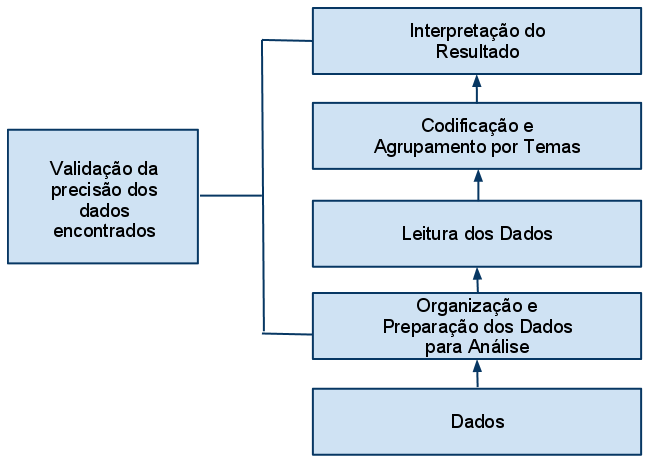
\includegraphics[scale=0.5]{analisedados}
  \caption{Processo de análise dos dados}
  \label{fig:analise-dados}
\end{figure}

 %% ------------------------------------------------------------------------- %%
\section{Validade e Confiabilidade do Estudo}
\label{sec:planejamento-validacao}

Para garantir a confiabilidade deste estudo, o pesquisador realizará os
seguintes procedimentos:

\begin{itemize}
	\item \textbf{Checar as transcrições}. O objetivo é garantir que nenhum erro
	óbvio foi cometido;

	\item \textbf{Verificação de pesquisador auxiliar}. Um pesquisador auxiliar
	checará se há algum desvio na definição dos códigos ou no significado dos códigos 
	durante o processo de codificação;
	
	\item \textbf{Rastreabilidade dos dados}. Todos os dados colhidos serão
	preservados em forma eletrônica.

\end{itemize}

A validade do estudo será garantida por alguns procedimentos executados pelos
pesquisadores, dentre eles:

\begin{itemize}
	\item \textbf{Triangulação diferentes fontes de dados}. A pesquisa é
	realizada em diferentes ambientes, com diferentes participantes e projetos,
	trazendo diferentes pontos de vista para dentro da análise;

	\item \textbf{Apresentar os resultados da pesquisa para os participantes e
	verificar se eles concordam com os resultados gerados}. Garantir que os
	participantes validem os dados encontrados diminui o viés do pesquisador;

	\item \textbf{Prover descrição rica e detalhada sobre o ambiente}. A riqueza
	dos detalhes mostra a qualidade do estudo, além de possibilitar a repetição do
	experimento por outros pesquisadores;

	\item \textbf{Esclarecer todos os possíveis vieses da pesquisa}. A pesquisa
	deixa claro quais são suas limitações. Todas elas são discutidos no Capítulo
	\ref{cap:ameacas}.

\end{itemize}

Em resumo, o principal meio de validação do estudo será o rico detalhamento dos
participantes, dos dados colhidos e instrumentos de coleta, de forma
que qualquer pesquisador interessado em replicar o experimento terá um
arcabouço sólido para comparação \cite{merriam-1998}. A análise de
dados também será relatada em detalhes para que os leitores tenham uma visão
acurada sobre o método utilizado na pesquisa. 
Além disso, essa pesquisa também é acompanhada pelo orientador do pesquisador,
que constantemente valida e discute os pontos levantados nesse planejamento.

%% ------------------------------------------------------------------------- %%
\section{Papel do Pesquisador}
\label{sec:planejamento-papel}

O pesquisador tem como papel fundamental participar do processo de captura dos
dados, bem como seu preparo e interpretação final.
Creswell \cite{creswell}, citando Locke \cite{locke}, lembra
que a contribuição do investigador para o contexto da pesquisa pode ser útil e
positiva ao invés de prejudicial. Além do mais, o pesquisador é responsável por
identificar todos os valores pessoais, pressuposições e vieses desse estudo.

O pesquisador tem formação em Ciência da Computação, e desenvolve software há 8
anos. Pratica TDD diariamente nos últimos 3 anos, e possui profundos
conhecimentos teóricos e práticos sobre orientação a objetos e métodos ágeis.
Além disso, o pesquisador palestrou sobre TDD em eventos da indústria brasileira
de desenvolvimento de software, como a Agile Brazil 2010, o .NET Architects
2010, e o QCON São Paulo 2010. O pesquisador acredita que sua experiência nessas
áreas aumentam sua capacidade de análise dos efeitos de TDD no design de sistemas 
orientados a objetos.

%% ------------------------------------------------------------------------- %%
\section{Problemas Éticos}
\label{sec:planejamento-etica}

Essa pesquisa poderá revelar problemas nas empresas selecionadas, como problemas
no design do software, na qualidade dos seus desenvolvedores, entre outros. 
Por esse motivo, todos os dados colhidos pelo pesquisador serão mantidos em
sigilo e todos os nomes de desenvolvedores e projetos omitidos, conforme acordo 
assinado entre o pesquisador e a empresa.

%% ------------------------------------------------------------------------- %%
\section{Resultados Esperados}
\label{sec:planejamento-resultados-esperados}

O objetivo desta pesquisa é entender, de maneira satisfatória, a influência de 
TDD no design de sistemas orientados a objetos, obtendo o ponto de vista dos 
desenvolvedores que a praticam diariamente. Conforme discutido nos trabalhos 
relacionados, muitos pesquisas já foram feitas, mas poucas discutem os motivos 
e as razões de TDD influenciar no design.

%% ------------------------------------------------------------------------- %%
\section{Estudo piloto}

% TODO: estudo piloto